
%% bare_conf.tex
%% V1.4b
%% 2015/08/26
%% by Michael Shell
%% See:
%% http://www.michaelshell.org/
%% for current contact information.
%%
%% This is a skeleton file demonstrating the use of IEEEtran.cls
%% (requires IEEEtran.cls version 1.8b or later) with an IEEE
%% conference paper.
%%
%% Support sites:
%% http://www.michaelshell.org/tex/ieeetran/
%% http://www.ctan.org/pkg/ieeetran
%% and
%% http://www.ieee.org/

%%*************************************************************************
%% Legal Notice:
%% This code is offered as-is without any warranty either expressed or
%% implied; without even the implied warranty of MERCHANTABILITY or
%% FITNESS FOR A PARTICULAR PURPOSE! 
%% User assumes all risk.
%% In no event shall the IEEE or any contributor to this code be liable for
%% any damages or losses, including, but not limited to, incidental,
%% consequential, or any other damages, resulting from the use or misuse
%% of any information contained here.
%%
%% All comments are the opinions of their respective authors and are not
%% necessarily endorsed by the IEEE.
%%
%% This work is distributed under the LaTeX Project Public License (LPPL)
%% ( http://www.latex-project.org/ ) version 1.3, and may be freely used,
%% distributed and modified. A copy of the LPPL, version 1.3, is included
%% in the base LaTeX documentation of all distributions of LaTeX released
%% 2003/12/01 or later.
%% Retain all contribution notices and credits.
%% ** Modified files should be clearly indicated as such, including  **
%% ** renaming them and changing author support contact information. **
%%*************************************************************************


% *** Authors should verify (and, if needed, correct) their LaTeX system  ***
% *** with the testflow diagnostic prior to trusting their LaTeX platform ***
% *** with production work. The IEEE's font choices and paper sizes can   ***
% *** trigger bugs that do not appear when using other class files.       ***                          ***
% The testflow support page is at:
% http://www.michaelshell.org/tex/testflow/



\documentclass[conference]{mnmc-format}
% Some Computer Society conferences also require the compsoc mode option,
% but others use the standard conference format.
%
% If IEEEtran.cls has not been installed into the LaTeX system files,
% manually specify the path to it like:
% \documentclass[conference]{../sty/IEEEtran}

\IEEEoverridecommandlockouts



% Some very useful LaTeX packages include:
% (uncomment the ones you want to load)


% *** MISC UTILITY PACKAGES ***
%


\usepackage{siunitx}
%\usepackage{ifpdf}
% Heiko Oberdiek's ifpdf.sty is very useful if you need conditional
% compilation based on whether the output is pdf or dvi.
% usage:
% \ifpdf
%   % pdf code
% \else
%   % dvi code
% \fi
% The latest version of ifpdf.sty can be obtained from:
% http://www.ctan.org/pkg/ifpdf
% Also, note that IEEEtran.cls V1.7 and later provides a builtin
% \ifCLASSINFOpdf conditional that works the same way.
% When switching from latex to pdflatex and vice-versa, the compiler may
% have to be run twice to clear warning/error messages.






% *** CITATION PACKAGES ***
%
\usepackage{cite}
% cite.sty was written by Donald Arseneau
% V1.6 and later of IEEEtran pre-defines the format of the cite.sty package
% \cite{} output to follow that of the IEEE. Loading the cite package will
% result in citation numbers being automatically sorted and properly
% "compressed/ranged". e.g., [1], [9], [2], [7], [5], [6] without using
% cite.sty will become [1], [2], [5]--[7], [9] using cite.sty. cite.sty's
% \cite will automatically add leading space, if needed. Use cite.sty's
% noadjust option (cite.sty V3.8 and later) if you want to turn this off
% such as if a citation ever needs to be enclosed in parenthesis.
% cite.sty is already installed on most LaTeX systems. Be sure and use
% version 5.0 (2009-03-20) and later if using hyperref.sty.
% The latest version can be obtained at:
% http://www.ctan.org/pkg/cite
% The documentation is contained in the cite.sty file itself.






% *** GRAPHICS RELATED PACKAGES ***
%
\usepackage{graphicx}
%\ifCLASSINFOpdf
\usepackage{subfigure}
  % \usepackage[pdftex]{graphicx}
  % declare the path(s) where your graphic files are
  % \graphicspath{{../pdf/}{../jpeg/}}
  % and their extensions so you won't have to specify these with
  % every instance of \includegraphics
  % \DeclareGraphicsExtensions{.pdf,.jpeg,.png}
%\else
  % or other class option (dvipsone, dvipdf, if not using dvips). graphicx
  % will default to the driver specified in the system graphics.cfg if no
  % driver is specified.
  % \usepackage[dvips]{graphicx}
  % declare the path(s) where your graphic files are
  % \graphicspath{{../eps/}}
  % and their extensions so you won't have to specify these with
  % every instance of \includegraphics
  % \DeclareGraphicsExtensions{.eps}
%\fi
% graphicx was written by David Carlisle and Sebastian Rahtz. It is
% required if you want graphics, photos, etc. graphicx.sty is already
% installed on most LaTeX systems. The latest version and documentation
% can be obtained at: 
% http://www.ctan.org/pkg/graphicx
% Another good source of documentation is "Using Imported Graphics in
% LaTeX2e" by Keith Reckdahl which can be found at:
% http://www.ctan.org/pkg/epslatex
%
% latex, and pdflatex in dvi mode, support graphics in encapsulated
% postscript (.eps) format. pdflatex in pdf mode supports graphics
% in .pdf, .jpeg, .png and .mps (metapost) formats. Users should ensure
% that all non-photo figures use a vector format (.eps, .pdf, .mps) and
% not a bitmapped formats (.jpeg, .png). The IEEE frowns on bitmapped formats
% which can result in "jaggedy"/blurry rendering of lines and letters as
% well as large increases in file sizes.
%
% You can find documentation about the pdfTeX application at:
% http://www.tug.org/applications/pdftex





% *** MATH PACKAGES ***
%
\usepackage{amsmath}
\usepackage{amssymb} % this enables the square symbol

% A popular package from the American Mathematical Society that provides
% many useful and powerful commands for dealing with mathematics.
%
% Note that the amsmath package sets \interdisplaylinepenalty to 10000
% thus preventing page breaks from occurring within multiline equations. Use:
%\interdisplaylinepenalty=2500
% after loading amsmath to restore such page breaks as IEEEtran.cls normally
% does. amsmath.sty is already installed on most LaTeX systems. The latest
% version and documentation can be obtained at:
% http://www.ctan.org/pkg/amsmath





% *** SPECIALIZED LIST PACKAGES ***
%
%\usepackage{algorithmic}
% algorithmic.sty was written by Peter Williams and Rogerio Brito.
% This package provides an algorithmic environment fo describing algorithms.
% You can use the algorithmic environment in-text or within a figure
% environment to provide for a floating algorithm. Do NOT use the algorithm
% floating environment provided by algorithm.sty (by the same authors) or
% algorithm2e.sty (by Christophe Fiorio) as the IEEE does not use dedicated
% algorithm float types and packages that provide these will not provide
% correct IEEE style captions. The latest version and documentation of
% algorithmic.sty can be obtained at:
% http://www.ctan.org/pkg/algorithms
% Also of interest may be the (relatively newer and more customizable)
% algorithmicx.sty package by Szasz Janos:
% http://www.ctan.org/pkg/algorithmicx




% *** ALIGNMENT PACKAGES ***
%
%\usepackage{array}
% Frank Mittelbach's and David Carlisle's array.sty patches and improves
% the standard LaTeX2e array and tabular environments to provide better
% appearance and additional user controls. As the default LaTeX2e table
% generation code is lacking to the point of almost being broken with
% respect to the quality of the end results, all users are strongly
% advised to use an enhanced (at the very least that provided by array.sty)
% set of table tools. array.sty is already installed on most systems. The
% latest version and documentation can be obtained at:
% http://www.ctan.org/pkg/array


% IEEEtran contains the IEEEeqnarray family of commands that can be used to
% generate multiline equations as well as matrices, tables, etc., of high
% quality.




% *** SUBFIGURE PACKAGES ***
%\ifCLASSOPTIONcompsoc
%  \usepackage[caption=false,font=normalsize,labelfont=sf,textfont=sf]{subfig}
%\else
%  \usepackage[caption=false,font=footnotesize]{subfig}
%\fi
% subfig.sty, written by Steven Douglas Cochran, is the modern replacement
% for subfigure.sty, the latter of which is no longer maintained and is
% incompatible with some LaTeX packages including fixltx2e. However,
% subfig.sty requires and automatically loads Axel Sommerfeldt's caption.sty
% which will override IEEEtran.cls' handling of captions and this will result
% in non-IEEE style figure/table captions. To prevent this problem, be sure
% and invoke subfig.sty's "caption=false" package option (available since
% subfig.sty version 1.3, 2005/06/28) as this is will preserve IEEEtran.cls
% handling of captions.
% Note that the Computer Society format requires a larger sans serif font
% than the serif footnote size font used in traditional IEEE formatting
% and thus the need to invoke different subfig.sty package options depending
% on whether compsoc mode has been enabled.
%
% The latest version and documentation of subfig.sty can be obtained at:
% http://www.ctan.org/pkg/subfig




% *** FLOAT PACKAGES ***
%
%\usepackage{fixltx2e}
% fixltx2e, the successor to the earlier fix2col.sty, was written by
% Frank Mittelbach and David Carlisle. This package corrects a few problems
% in the LaTeX2e kernel, the most notable of which is that in current
% LaTeX2e releases, the ordering of single and double column floats is not
% guaranteed to be preserved. Thus, an unpatched LaTeX2e can allow a
% single column figure to be placed prior to an earlier double column
% figure.
% Be aware that LaTeX2e kernels dated 2015 and later have fixltx2e.sty's
% corrections already built into the system in which case a warning will
% be issued if an attempt is made to load fixltx2e.sty as it is no longer
% needed.
% The latest version and documentation can be found at:
% http://www.ctan.org/pkg/fixltx2e


%\usepackage{stfloats}
% stfloats.sty was written by Sigitas Tolusis. This package gives LaTeX2e
% the ability to do double column floats at the bottom of the page as well
% as the top. (e.g., "\begin{figure*}[!b]" is not normally possible in
% LaTeX2e). It also provides a command:
%\fnbelowfloat
% to enable the placement of footnotes below bottom floats (the standard
% LaTeX2e kernel puts them above bottom floats). This is an invasive package
% which rewrites many portions of the LaTeX2e float routines. It may not work
% with other packages that modify the LaTeX2e float routines. The latest
% version and documentation can be obtained at:
% http://www.ctan.org/pkg/stfloats
% Do not use the stfloats baselinefloat ability as the IEEE does not allow
% \baselineskip to stretch. Authors submitting work to the IEEE should note
% that the IEEE rarely uses double column equations and that authors should try
% to avoid such use. Do not be tempted to use the cuted.sty or midfloat.sty
% packages (also by Sigitas Tolusis) as the IEEE does not format its papers in
% such ways.
% Do not attempt to use stfloats with fixltx2e as they are incompatible.
% Instead, use Morten Hogholm'a dblfloatfix which combines the features
% of both fixltx2e and stfloats:
%
% \usepackage{dblfloatfix}
% The latest version can be found at:
% http://www.ctan.org/pkg/dblfloatfix

\usepackage{siunitx}


% *** PDF, URL AND HYPERLINK PACKAGES ***
%
%\usepackage{url}
% url.sty was written by Donald Arseneau. It provides better support for
% handling and breaking URLs. url.sty is already installed on most LaTeX
% systems. The latest version and documentation can be obtained at:
% http://www.ctan.org/pkg/url
% Basically, \url{my_url_here}.
\usepackage{xcolor}
\usepackage{graphicx}


%\usepackage{todonotes}

\newcommand\todo[1]{\textcolor{red}{\textbf{TO DO: #1}}}
\newcommand\lorem{\textcolor{green}{\textbf{Lorem ipsum dolor sit amet, consectetuer adipiscing elit.Etiam lobortis facilisis sem. Nullam nec mi et neque pharetrasollicitudin. Praesent imperdiet mi nec ante. Donec ullamcor-per, felis non sodales commodo, lectus velit ultrices augue,a dignissim nibh lectus placerat pede. Vivamus nunc nunc,molestie ut, ultricies vel, semper in, velit. Ut porttitor. Praesentin sapien. Lorem ipsum dolor sit amet, consectetuer adipiscingelit. Duis fringilla tristique neque. Sed interdum libero utmetus. Pellentesque placerat. Nam rutrum augue a leo. Morbised elit sit amet ante lobortis sollicitudin. Praesent blanditblandit mauris. Praesent lectus tellus, aliquet aliquam, luctusa, egestas a, turpis. Mauris lacinia lorem sit amet ipsum. Nuncquis urna dictum turpis accumsan semper.}}}

% *** Do not adjust lengths that control margins, column widths, etc. ***
% *** Do not use packages that alter fonts (such as pslatex).         ***
% There should be no need to do such things with IEEEtran.cls V1.6 and later.
% (Unless specifically asked to do so by the journal or conference you plan
% to submit to, of course. )


% correct bad hyphenation here
\hyphenation{op-tical net-works semi-conduc-tor}


\begin{document}
%
% paper title
% Titles are generally capitalized except for words such as a, an, and, as,
% at, but, by, for, in, nor, of, on, or, the, to and up, which are usually
% not capitalized unless they are the first or last word of the title.
% Linebreaks \\ can be used within to get better formatting as desired.
% Do not put math or special symbols in the title.
\title{EE247 Final Project Report}


% author names and affiliations
% use a multiple column layout for up to three different
% affiliations

\author{\IEEEauthorblockN{Kenny Tan, Aniket Tolpadi, Zhizheng Qiao, Tianhua Xia, Rachel Zoll\\}
\IEEEauthorblockA{Department of Electrical Engineering and Computer Sciences, University of California Berkeley, Berkeley, CA 94720\\
Email: \{kennyftan, atolpadi, xiatianhua970512, qiaozhizheng, rachelzoll\}@berkeley.edu}}
    

% conference papers do not typically use \thanks and this command
% is locked out in conference mode. If really needed, such as for
% the acknowledgment of grants, issue a \IEEEoverridecommandlockouts
% after \documentclass

% for over three affiliations, or if they all won't fit within the width
% of the page, use this alternative format:
% 
%\author{\IEEEauthorblockN{Michael Shell\IEEEauthorrefmark{1},
%Homer Simpson\IEEEauthorrefmark{2},
%James Kirk\IEEEauthorrefmark{3}, 
%Montgomery Scott\IEEEauthorrefmark{3} and
%Eldon Tyrell\IEEEauthorrefmark{4}}
%\IEEEauthorblockA{\IEEEauthorrefmark{1}School of Electrical and Computer Engineering\\
%Georgia Institute of Technology,
%Atlanta, Georgia 30332--0250\\ Email: see http://www.michaelshell.org/contact.html}
%\IEEEauthorblockA{\IEEEauthorrefmark{2}Twentieth Century Fox, Springfield, USA\\
%Email: homer@thesimpsons.com}
%\IEEEauthorblockA{\IEEEauthorrefmark{3}Starfleet Academy, San Francisco, California 96678-2391\\
%Telephone: (800) 555--1212, Fax: (888) 555--1212}
%\IEEEauthorblockA{\IEEEauthorrefmark{4}Tyrell Inc., 123 Replicant Street, Los Angeles, California 90210--4321}}




% use for special paper notices
%\IEEEspecialpapernotice{(Invited Paper)}




% make the title area
\maketitle

% As a general rule, do not put math, special symbols or citations
% in the abstract
%\IEEEtitleabstractindextext{%
\begin{abstract}
   Abstract goes here
   \todo{Write abstract}
    
\end{abstract}

% Note that keywords are not normally used for peerreview papers.
%\begin{IEEEkeywords}
%Computer Society, IEEE, IEEEtran, journal, \LaTeX, paper, template.
%\end{IEEEkeywords}}




% no keywords



% For peer review papers, you can put extra information on the cover
% page as needed:
% \ifCLASSOPTIONpeerreview
% \begin{center} \bfseries EDICS Category: 3-BBND \end{center}
% \fi
%
% For peerreview papers, this IEEEtran command inserts a page break and
% creates the second title. It will be ignored for other modes.
\IEEEpeerreviewmaketitle


\section{Introduction}

%~\cite{Contreras2017,Vitale2018,Muthuswamy2005,Tas2003a,Feingold2018,Karpelson2008,Patel2016,Kozai2012,Lecomte2017,Massey2018,Chen2017a,Guitchounts2013,Merrill2005,Jackson2010,Deepthi2010,Welkenhuysen2011,BeMent1986,Gillis2017,Reitboeck1983,Rousche1998,Schindler2017,Clark2010a,Leis2000,Patel2015,Muthuswamy2005a,Yeh2002,Penskiy2013,Reichert2007,Bernatchez1996,Sanders2000}
Intro goes here
\todo{write this section}
    
\section{Materials and Methods}


% \begin{figure}[!htb]
%     \centering
%     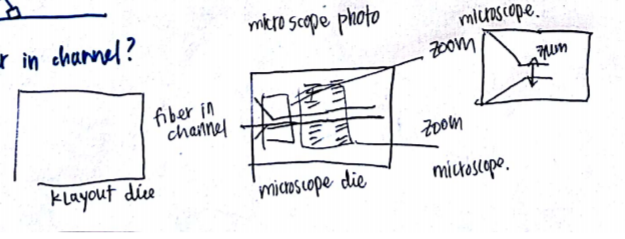
\includegraphics[width=1\columnwidth]{images/cartoon/die_klayout.png}
%     \vspace{0mm}
%     \caption{Layout and fabricated designs. (a) Microelectrode actuator design in layout. (b) The fabricated design. (c) Detail showing insertion funnel for loading carbon fibers. (d) Detail showing angled arm design with carbon fiber in the channel.}
%     \label{fig:die-klayout}
% \end{figure}


\begin{figure}[]
    \centering
    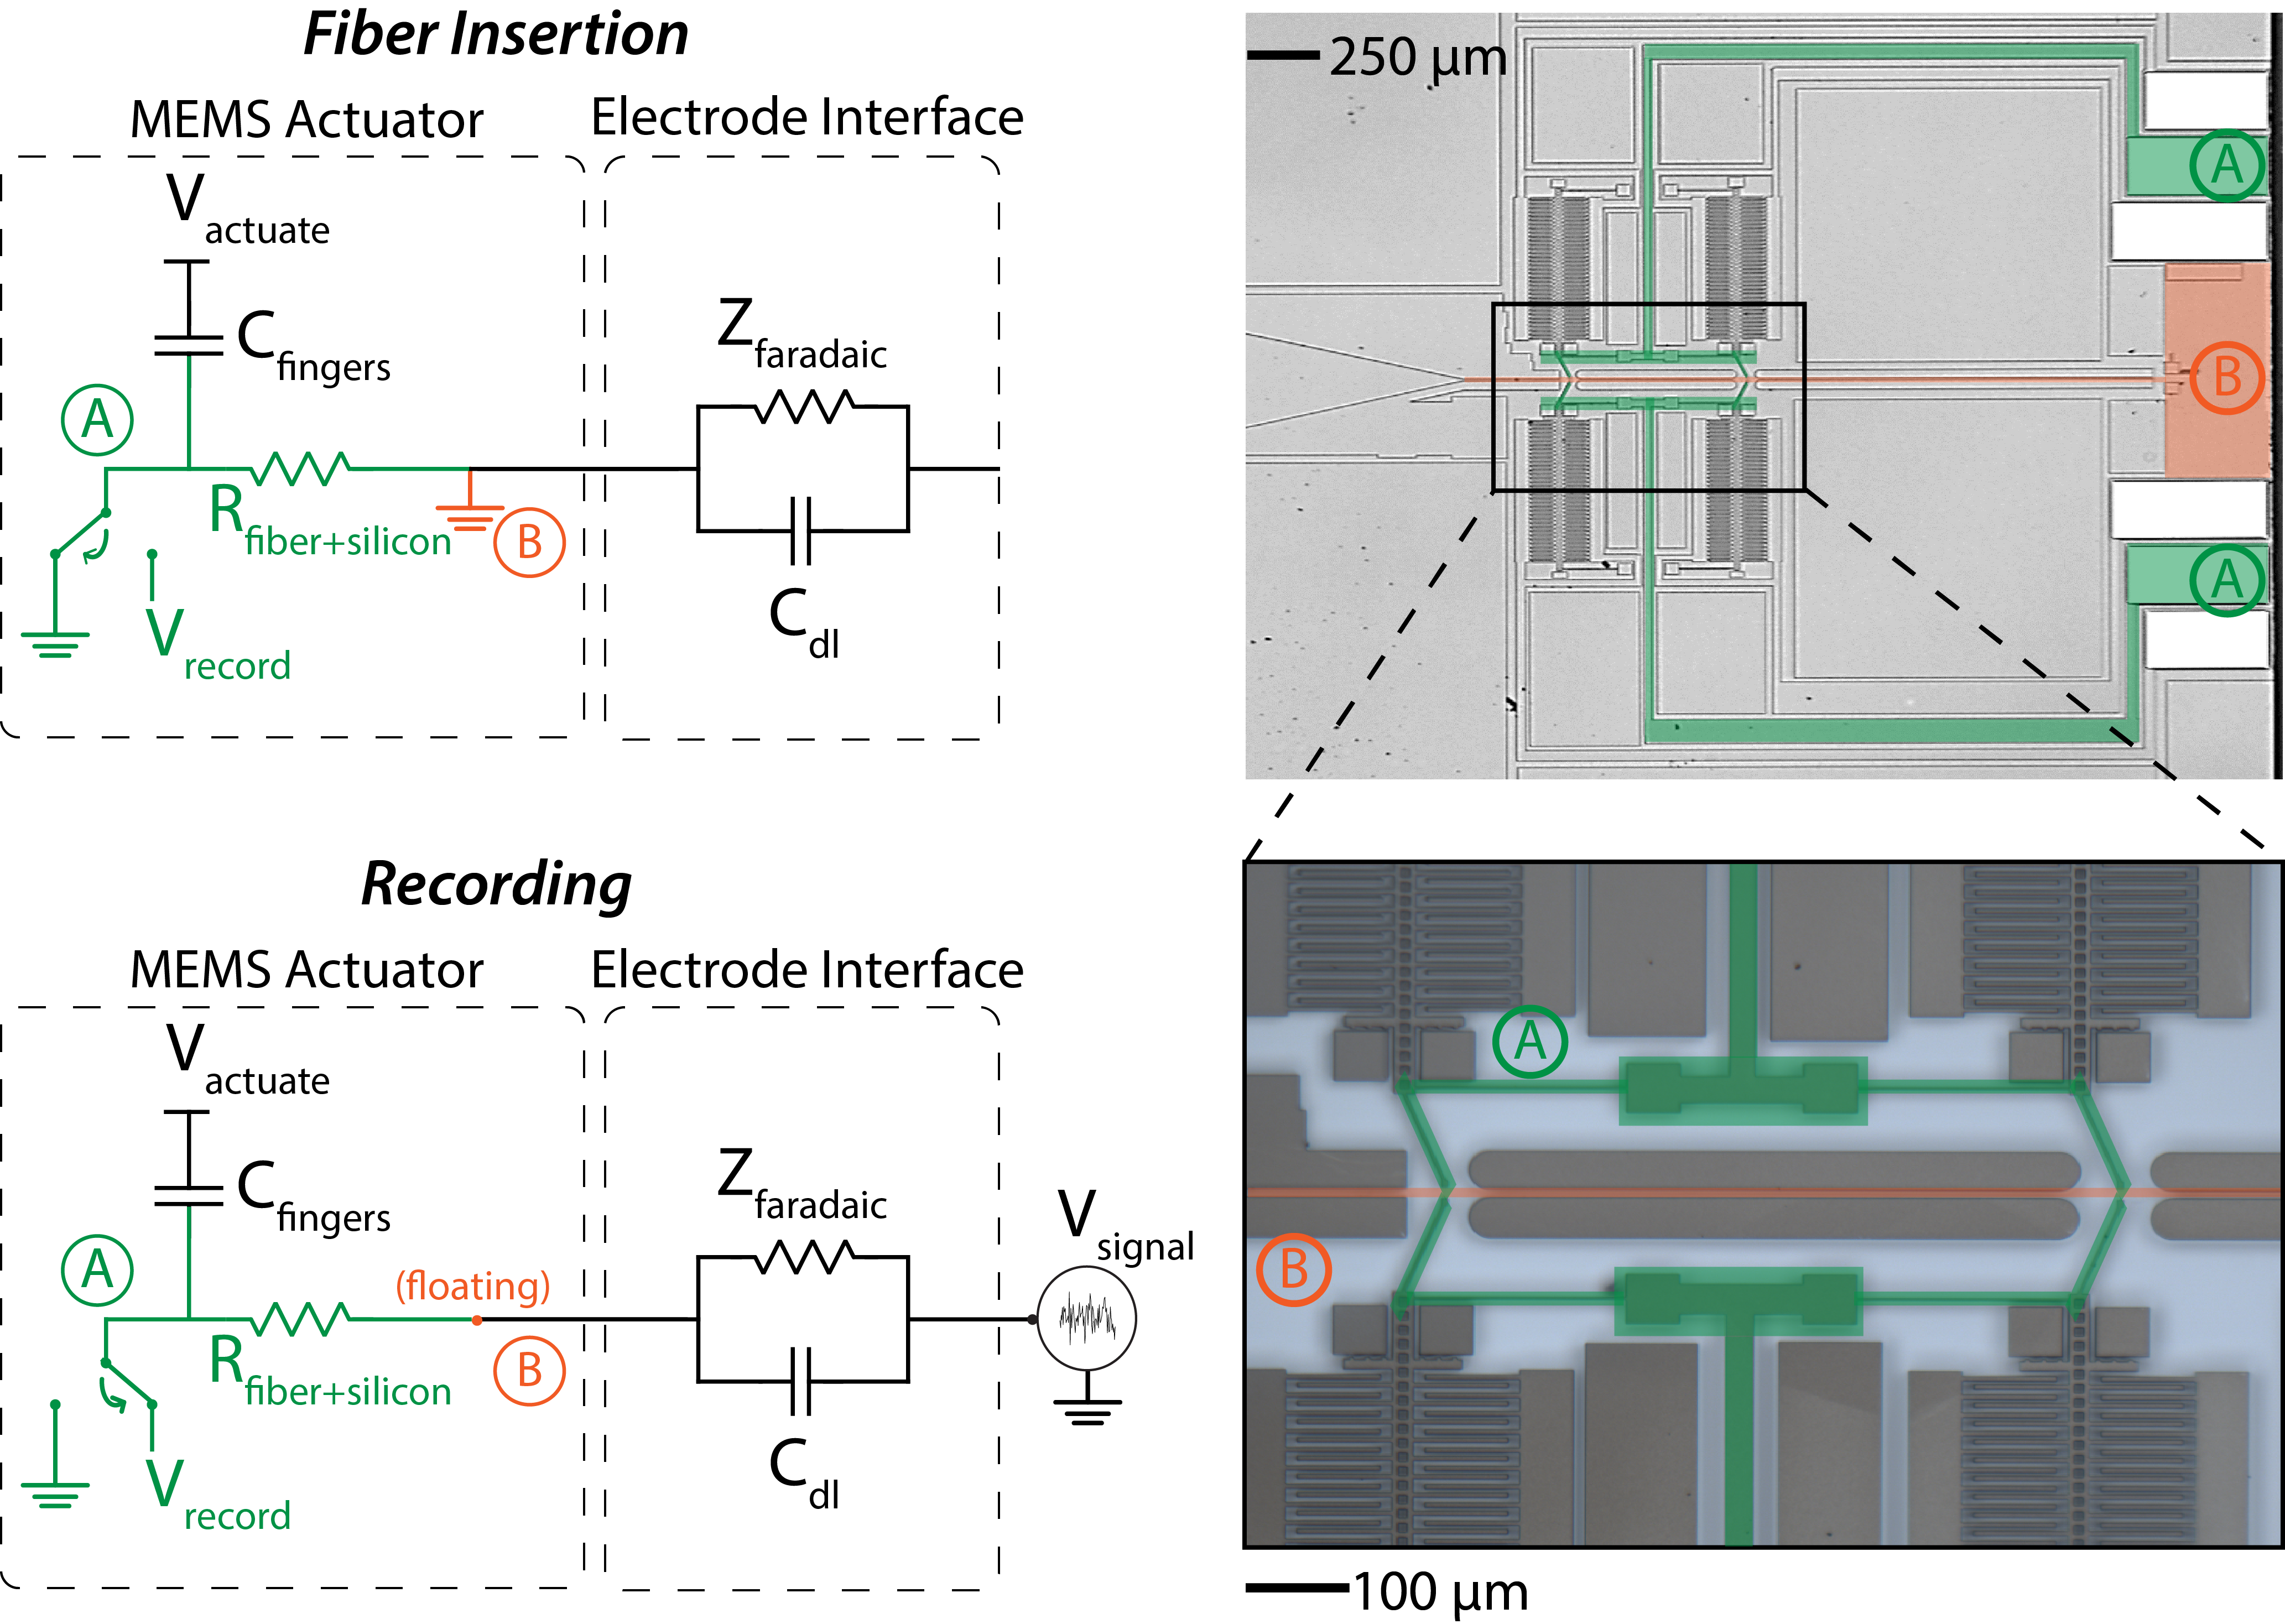
\includegraphics[width=\columnwidth]{images/cartoon-2stages-dd.png}
    \caption{Left: Equivalent circuit models of the device. During fiber insertion (top), the electrostatic actuator pushes the fiber forwards in channel. During recording (bottom), neural signals are captured by closing all four angled arms until they contact the carbon fiber. Electrically connected segments have been labelled and highlighted. ``A'', green, represents the silicon traces and angled arms which contact the carbon fiber; ``B'', orange, represents the carbon fiber channel and substrate. Right: Image of the device, with inset shown at bottom.}
    \label{fig:cartoon-2states}
\end{figure}

\subsection{Theory of Operation}
\todo{update this section}

    %\todo{Make sure figures are all spaced appropriately}
    \subsubsection{Fiber Insertion}

    In this work, we designed a MEMS actuator containing an electrostatic motor with angled arms, as in~\cite{Penskiy2013, Schindler2017}. The electrostatic motors presented here are capable of producing millinewton forces over many millimeters of travel~\cite{Yeh2002, Penskiy2013, Contreras2017, Schindler2017}, sufficient for the penetration forces (calculated to be on the order of hundreds of micronewtons for this electrode style) and depths necessary for most applications~\cite{Massey2018,Patel2016,Kozai2012}. In prior work, these actuators have been used to advance \SI{7.2}{\micro\meter} carbon fibers in air, but have not been characterized for their mechanical insertion and electrical characteristics in the context of neural recording \cite{Schindler2017}.
    
    Each actuation cycle of the electrostatic motor pushes the fiber a small distance. Motion is achieved by applying voltage to an interdigitated set of capacitive fingers. Initially, one set of fingers is grounded, while the other set is held at V$_{actuate}$. This electrostatic force causes the interdigitated capacitive fingers to pull in towards one another, in turn pushing out a set of flexible angled arms which grip the carbon fiber. To disengage the flexible arms from the carbon fiber, both sets of capacitive fingers are grounded and a spring pulls the capacitive fingers apart. 
    
    By using two such actuators to perform a cyclic motion in which the angled arms come into contact with the carbon fiber, move it forwards one step, disengage, and return to their initial position, the motor accumulates small steps which eventually advance the microelectrode over a large distance. For more details on actuation, see~\cite{Penskiy2013}.

    % then translated to the carbon fiber via two sets of flexible angled arms, which correspondingly grip and release the fiber in anti-phase to accumulate small forwards motions. As seen in \todo{some figure in this text which diagrams gap closers actuating vertically, shuttle pushed horizontally}, the movement of GCAs is perpendicular to that of the carbon fiber; however, the angled arm applies force in both the transverse and longitudinal directions. Transverse forces produced by opposite sets of actuators are cancelled out, producing a net longitudinal force. Silicon springs provide a restoring force when high-voltage is removed~\cite{Penskiy2013}. 

    % Discussion of connections
    
    Fig.~\ref{fig:cartoon-2states} shows equivalent circuit diagrams (left) and corresponding images of the device (right) with electrically connected segments labelled and highlighted.
    
    During insertion of a fiber (Fig.~\ref{fig:cartoon-2states}, top left), the silicon angled arms and one set of capacitive fingers in each actuator are tied to ground (highlighted in green, ``A''). The other set of capacitive fingers alternates between V$_{actuate}$ and ground, dictating whether the angled arms are in contact with or disengaged from the carbon fiber. The substrate (highlighted in orange, ``B'') is also grounded to prevent released silicon structures from electrostatically pulling in to the substrate.
    
    In Fig.~\ref{fig:cartoon-2states} (top right), the green highlighted regions indicate the signal path from the wirebond pads, through the silicon traces, to the angled arms which contact the carbon fiber. The orange highlighted regions indicate the substrate connection and location of a carbon fiber within the channel. Fig.~\ref{fig:cartoon-2states} (bottom right) shows an inset of the silicon traces and angled arms (green) which come in contact with the fiber, nominally held in place in the fiber channel (orange).

    When no voltage is applied to the actuator motor, the carbon fiber is not in contact with any silicon structure other than the substrate.
    
    \subsubsection{Recording}
    When recording signals from the electrode (Fig.~\ref{fig:cartoon-2states}, bottom left), all four angled arms make contact with the carbon fiber when a high voltage, V$_{actuate}$, is maintained across the capacitive fingers. These silicon arms, along with the corresponding silicon routing, form a signal path with which to record the neural signal. The path of impedance for this signal, from the tip of the carbon fiber in contact with the electrolyte to the external sensor circuity wire-bonded to the die, includes: parallel double-layer capacitance C$_{dl}$ and faradaic impedance Z$_{faradaic}$ at the electrode-electrolyte interface; carbon fiber impedance R$_{fiber+silicon}$; contact resistance between the carbon fiber and silicon angled arms; silicon traces; and wire bonds (all included in R$_{fiber+silicon}$). 
    
    The electrophysiological potential is recorded from the signal pad (green, ``A'') versus a reference electrode. The substrate and carbon fiber channel (orange, ``B'') are left floating to prevent grounding of the recorded signal. Although the voltage difference between the sets of capacitive fingers becomes V$_{actuate}-$V$_{signal}$ due to the micro-to-millivolt amplitude of neural recordings, this voltage is still sufficient to allow the angled arms to grip the fiber.

\subsection{Device Fabrication and Assembly}
    The MEMS actuator was fabricated with a two-mask silicon-on-insulator (SOI) process. Commercial SOI wafers consisting of a silicon substrate (\SI{550}{\micro\meter}), buried oxide layer (\SI{2}{\micro\meter}), and a device silicon layer (\SI{40}{\micro\meter}, \SI{3250}{\ohm}/$\square$), were used for all devices. First, aluminium was evaporated onto the wirebond sites to improve bond adhesion. Device silicon was lithographically patterned and etched using a deep reactive ion etch (DRIE). A subsequently patterned through-etch of the silicon substrate layer, also via DRIE, served to singulate the devices. Finally, a timed vapor HF etch was used to release the structures. The fabricated device is shown in Fig.~\ref{fig:die-photo} and Fig.~\ref{fig:cartoon-2states} (right).

    Electrical connections were made by wirebonding signal wires from the chip to an off-chip set of interconnects. A substrate grounding wire and the chip were held in place with silver epoxy. Placement of the fiber within the channel was achieved by adhering a fiber to a silicone-coated tungsten micromanipulator probe tip. The probe tip and carbon fiber assembly was aligned to the left of the device layer funnel, lowered to the correct height above the chip, and inserted into the channel. %Care was taken to prevent silver epoxy from shorting along the gold-coated interconnects.
    %The epoxy was cured at \SI{150}{\celsius} for \SI{10}{\minute}.
    %with \SIrange{8}{10}{\milli\meter} of carbon fiber extended beyond the edge of the probe tip. 
    %The entire chip assembly, including glass slide surface, grounding wire, MEMS chip, gold interconnects and wirebonds, is mounted on a vacuum chuck to provide stability during fiber insertion. 
    
    %Finally, the probe tip was separated from the fiber by lifting it out of plane.
    The chip is \SI{4.5}{\milli\meter} by \SI{3.5}{\milli\meter}, and has a mass of \SI{22}{\milli\gram}. The actuator/motor area is approximately \SI{1.5}{\square\milli\meter}.
    
\begin{figure}[t]
\centering
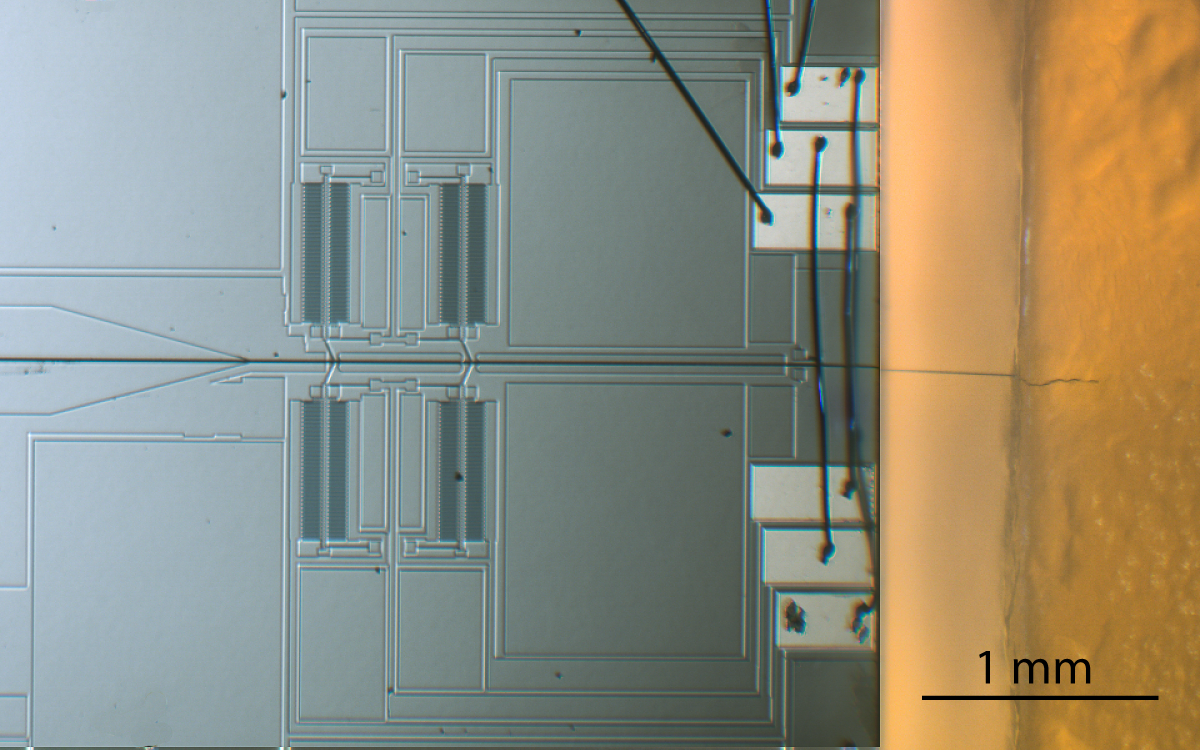
\includegraphics[width=\columnwidth]{images/CompositeFin.png}
\caption{The MEMS actuator and a \SI{7.2}{\micro\meter} diameter carbon fiber inserted approximately \SI{400}{\micro\meter} into the agar brain phantom.}
\label{fig:agar-push-composite}
\end{figure}

    
    
\section{Results and Discussion}

\begin{figure}[]
    \centering
    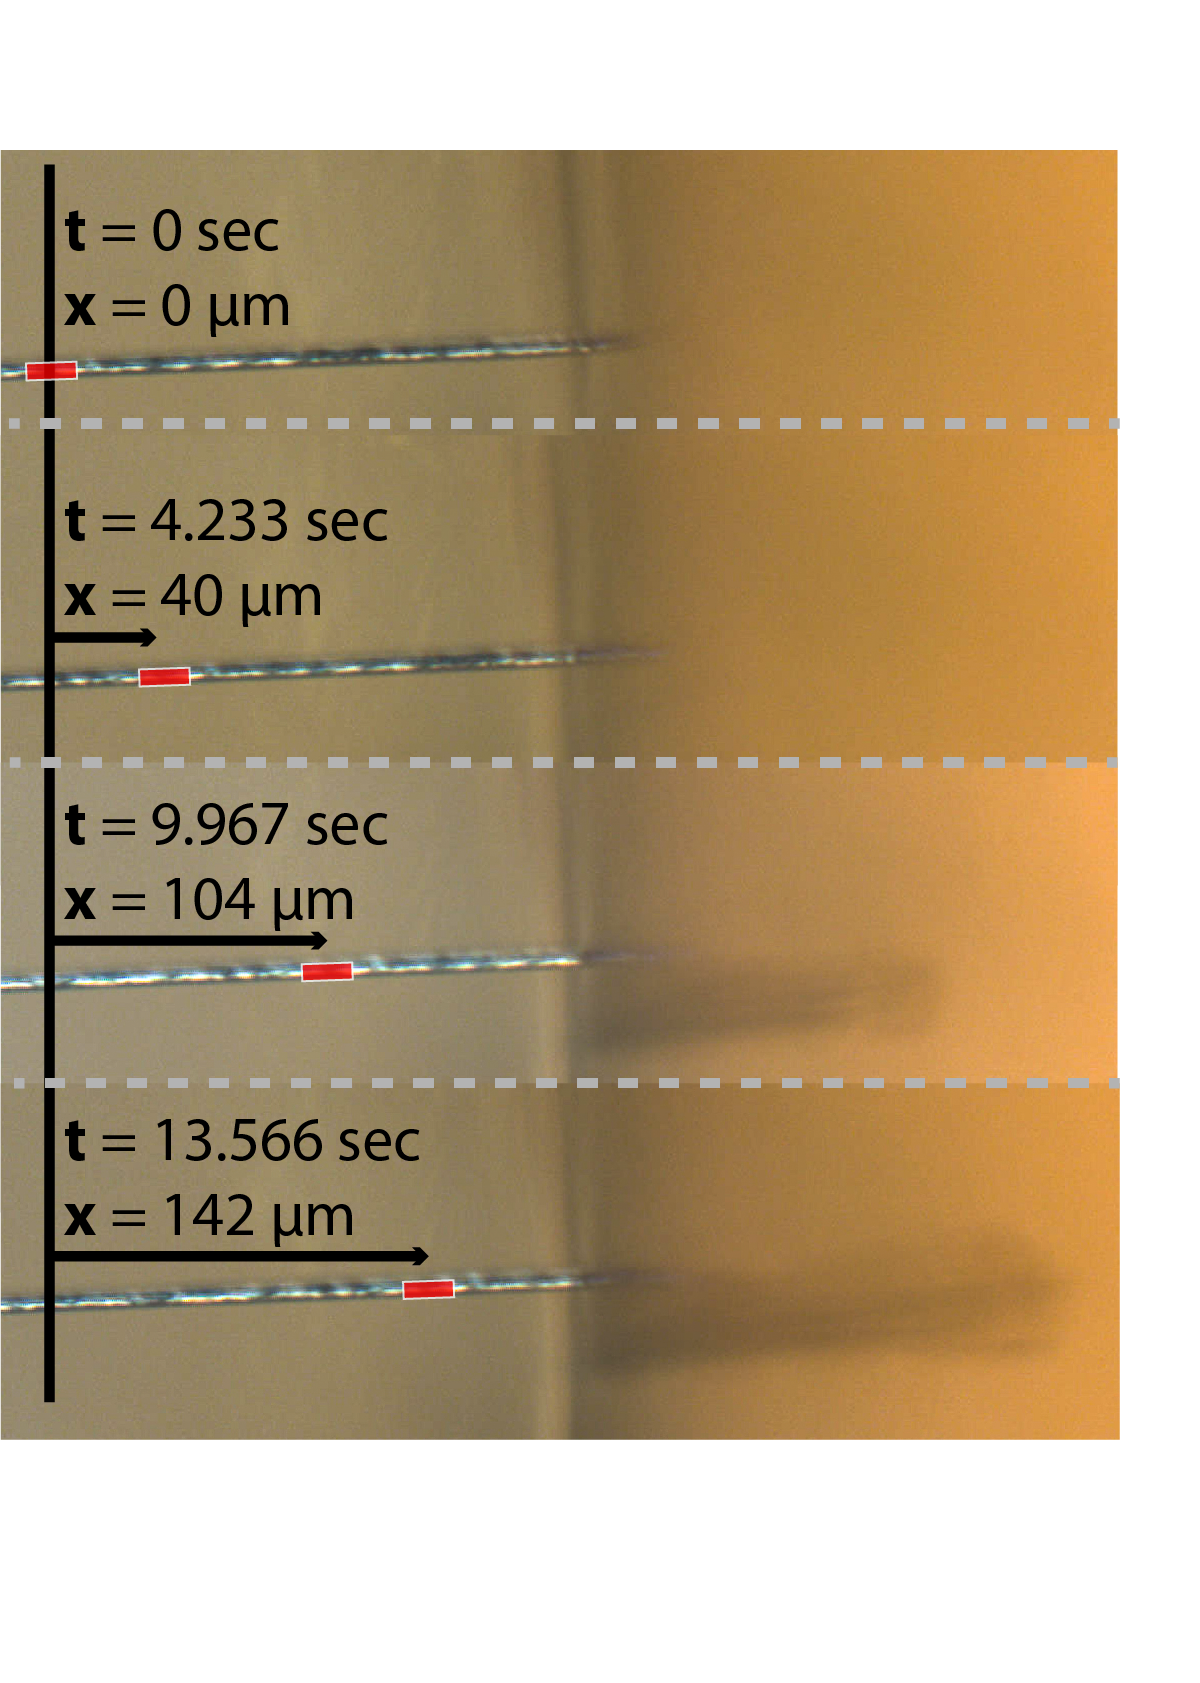
\includegraphics[width=0.8\columnwidth]{images/ProgressionCuts.png}
    \vspace{-1.1cm}
    \caption{Multiple close-up shots showing the insertion of a \SI{7.2}{\micro\meter} diameter carbon fiber into the brain phantom. The red dash indicates the same position on the carbon fiber between frames.}
    \label{fig:agar-push-frames}
\end{figure}

\todo{write this section}



\section{Conclusions and Future Work}
Conclusions and Future Work go here
\todo{write this section}
\section*{Acknowledgment}

We thank the Berkeley Sensor~\&~Actuator Center for support during this project. All fabrication was performed at the UC Berkeley Marvell Nanolab. The authors would also like to thank H. Gomez, J. Greenspun, K. Pister, and C. Schindler for their support throughout this project.



% An example of a floating figure using the graphicx package.
% Note that \label must occur AFTER (or within) \caption.
% For figures, \caption should occur after the \includegraphics.
% Note that IEEEtran v1.7 and later has special internal code that
% is designed to preserve the operation of \label within \caption
% even when the captionsoff option is in effect. However, because
% of issues like this, it may be the safest practice to put all your
% \label just after \caption rather than within \caption{}.
%
% Reminder: the "draftcls" or "draftclsnofoot", not "draft", class
% option should be used if it is desired that the figures are to be
% displayed while in draft mode.
%
%\begin{figure}[!t]
%\centering
%\includegraphics[width=2.5in]{myfigure}
% where an .eps filename suffix will be assumed under latex, 
% and a .pdf suffix will be assumed for pdflatex; or what has been declared
% via \DeclareGraphicsExtensions.
%\caption{Simulation results for the network.}
%\label{fig_sim}
%\end{figure}

% Note that the IEEE typically puts floats only at the top, even when this
% results in a large percentage of a column being occupied by floats.


% An example of a double column floating figure using two subfigures.
% (The subfig.sty package must be loaded for this to work.)
% The subfigure \label commands are set within each subfloat command,
% and the \label for the overall figure must come after \caption.
% \hfil is used as a separator to get equal spacing.
% Watch out that the combined width of all the subfigures on a 
% line do not exceed the text width or a line break will occur.
%
%\begin{figure*}[!t]
%\centering
%\subfloat[Case I]{\includegraphics[width=2.5in]{box}%
%\label{fig_first_case}}
%\hfil
%\subfloat[Case II]{\includegraphics[width=2.5in]{box}%
%\label{fig_second_case}}
%\caption{Simulation results for the network.}
%\label{fig_sim}
%\end{figure*}
%
% Note that often IEEE papers with subfigures do not employ subfigure
% captions (using the optional argument to \subfloat[]), but instead will
% reference/describe all of them (a), (b), etc., within the main caption.
% Be aware that for subfig.sty to generate the (a), (b), etc., subfigure
% labels, the optional argument to \subfloat must be present. If a
% subcaption is not desired, just leave its contents blank,
% e.g., \subfloat[].


% An example of a floating table. Note that, for IEEE style tables, the
% \caption command should come BEFORE the table and, given that table
% captions serve much like titles, are usually capitalized except for words
% such as a, an, and, as, at, but, by, for, in, nor, of, on, or, the, to
% and up, which are usually not capitalized unless they are the first or
% last word of the caption. Table text will default to \footnotesize as
% the IEEE normally uses this smaller font for tables.
% The \label must come after \caption as always.
%
%\begin{table}[!t]
%% increase table row spacing, adjust to taste
%\renewcommand{\arraystretch}{1.3}
% if using array.sty, it might be a good idea to tweak the value of
% \extrarowheight as needed to properly center the text within the cells
%\caption{An Example of a Table}
%\label{table_example}
%\centering
%% Some packages, such as MDW tools, offer better commands for making tables
%% than the plain LaTeX2e tabular which is used here.
%\begin{tabular}{|c||c|}
%\hline
%One & Two\\
%\hline
%Three & Four\\
%\hline
%\end{tabular}
%\end{table}


% Note that the IEEE does not put floats in the very first column
% - or typically anywhere on the first page for that matter. Also,
% in-text middle ("here") positioning is typically not used, but it
% is allowed and encouraged for Computer Society conferences (but
% not Coamputer Society journals). Most IEEE journals/conferences use
% top floats exclusively. 
% Note that, LaTeX2e, unlike IEEE journals/conferences, places
% footnotes above bottom floats. This can be corrected via the
% \fnbelowfloat command of the stfloats package.




% trigger a \newpage just before the given reference
% number - used to balance the columns on the last page
% adjust value as needed - may need to be readjusted if
% the document is modified later
%\IEEEtriggeratref{8}
% The "triggered" command can be changed if desired:
%\IEEEtriggercmd{\enlargethispage{-5in}}

% references section

% can use a bibliography generated by BibTeX as a .bbl file
% BibTeX documentation can be easily obtained at:
% http://mirror.ctan.org/biblio/bibtex/contrib/doc/
% The IEEEtran BibTeX style support page is at:
% http://www.michaelshell.org/tex/ieeetran/bibtex/
%\bibliographystyle{IEEEtran}
% argument is your BibTeX string definitions and bibliography database(s)
%\bibliography{IEEEabrv,../bib/paper}
%
% <OR> manually copy in the resultant .bbl file
% set second argument of \begin to the number of references
% (used to reserve space for the reference number labels box)
% \begin{thebibliography}
%\bibitem{IEEEhowto:kopka}
%H.~Kopka and P.~W. Daly, \emph{A Guide to \LaTeX}, 3rd~ed.\hskip 1em plus
%  0.5em minus 0.4em\relax Harlow, England: Addison-Wesley, 1999.
%\section*{References}
\bibliography{mnmc-conf}
\bibliographystyle{IEEEtran}


% \end{thebibliography}




% that's all folks
\end{document}


